\documentclass[12pt]{article}
\usepackage[margin=0.1in]{geometry}
\usepackage{arev}
\usepackage{pgfplots}
\pgfplotsset{compat=newest}

\begin{document}

% First example of the notes
\begin{figure}[hbt]
    \centering
    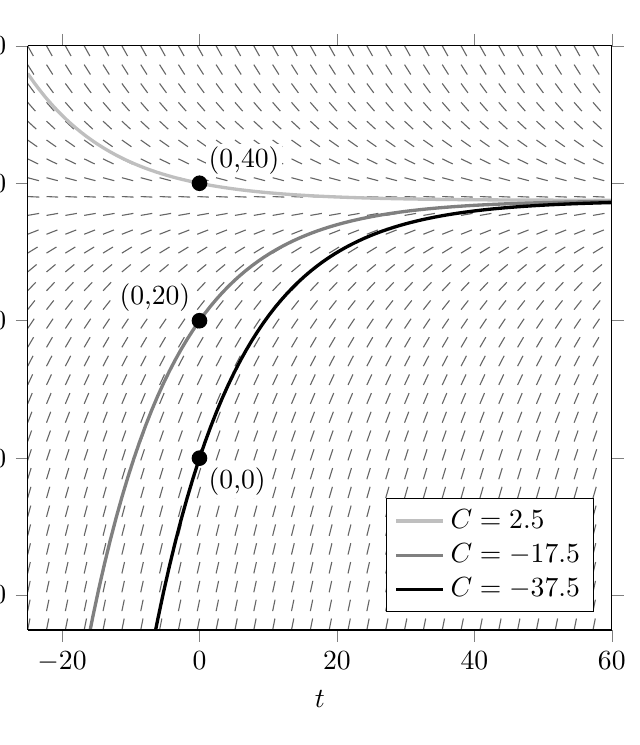
\begin{tikzpicture}[trim axis left, trim axis right] % options to centre correctly
        \def\dydx{3-0.08*y} % differential equation: dy/dx = f(x,y) => \def\dydx{f(x,y)}
        \newcommand\solution[1]{37.5+#1*exp(-0.08*x)} % general solution with integration constant c, given by #1

        % domain and tick settings - note domain is square, change in axis options if needed
        \def\domainMin{-25}
        \def\domainMax{60}
        \def\ticks{\domainMin+5,\domainMin+25,...,\domainMax} % define tick marks
        \pgfmathsetmacro\quiverScale{(\domainMax-\domainMin)/50}

        % #1: coordinates of node, #2: relative position of node label (can also be angle)
        \newcommand\labelledPoint[2]{\node[circle, fill, inner sep=2pt, label={[fill=white,distance=1pt,inner sep=1pt]#2:{(#1)}}] at (#1){}}

        \begin{axis}[view = {0}{90}, % set camera to point towards x-y plane
                     domain=\domainMin:\domainMax,
                     xmin=\domainMin, xmax=\domainMax,
                     ymin=\domainMin, ymax=\domainMax,
                     xlabel=$t$, ylabel=$w$,
                     xtick=\ticks, ytick=\ticks,
                     tick align=outside,
                     width=9cm, height=9cm,
                     legend pos=south east, legend cell align={left},
                     axis equal image]

            % plot unit length quivers with no head
            \addplot3[black!60, quiver={u=1/(sqrt((\dydx)^2+1)), v=(\dydx)/(sqrt((\dydx)^2+1)), scale arrows=\quiverScale}, samples=32, forget plot] (x,y,0);

            % plot initial points and corresponding solution curves
            \addplot[very thick, black!25, samples=100] plot (x,\solution{2.5});
            \labelledPoint{0,40}{above right};

            \addplot[very thick, black!50, samples=100] plot (x,\solution{-17.5});
            \labelledPoint{0,20}{above left};

            \addplot[very thick, black!100, samples=100] plot (x,\solution{-37.5});
            \labelledPoint{0,0}{below right};

            % add legend, ignoring quiver plot
            \legend{$C=2.5$, $C=-17.5$, $C=-37.5$}
        \end{axis}
    \end{tikzpicture}
    \caption{Slope field of $\frac{\mathrm{d}w}{\mathrm{d}t}=3-0.08w$, with general solution $w(t)=Ce^{-0.08t}+37.5$}
\end{figure}

% Second example of the notes
\begin{figure}[hbt]
    \centering
    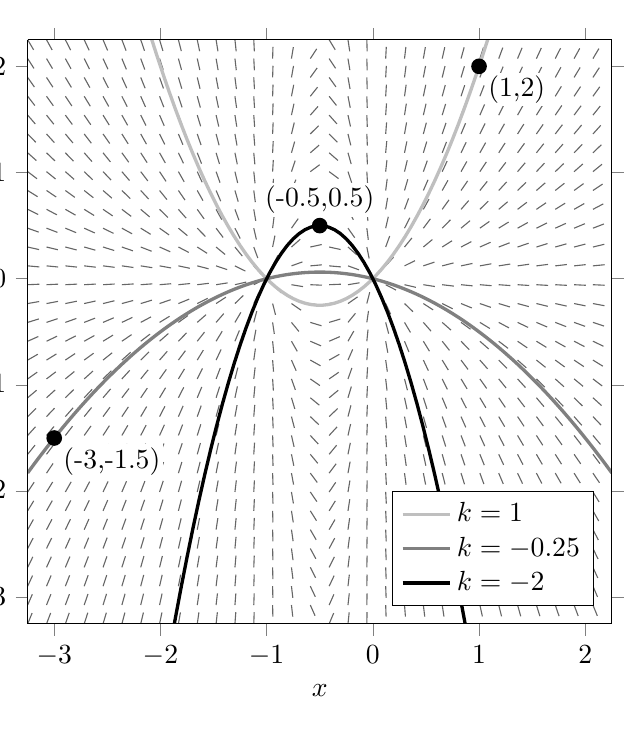
\begin{tikzpicture}[trim axis left, trim axis right] % options to centre correctly
        \def\dydx{(2*x+1)*y / (x^2+x)} % differential equation: dy/dx = f(x,y) => \def\dydx{f(x,y)}
        \newcommand\solution[1]{#1*(x^2+x)} % general solution with integration constant k, given by #1

        % domain and tick settings - note domain is square, change in axis options if needed
        \def\domainMin{-3.25}
        \def\domainMax{2.25}
        \def\ticks{\domainMin+0.25,...,\domainMax-0.25} % define tick marks
        \pgfmathsetmacro\quiverScale{(\domainMax-\domainMin)/50}

        % #1: coordinates of node, #2: relative position of node label (can also be angle)
        \newcommand\labelledPoint[2]{\node[circle, fill, inner sep=2pt, label={[fill=white,distance=1pt,inner sep=1pt]#2:{(#1)}}] at (#1){}}

        \begin{axis}[view = {0}{90}, % set camera to point towards x-y plane
                     domain=\domainMin:\domainMax,
                     xmin=\domainMin, xmax=\domainMax,
                     ymin=\domainMin, ymax=\domainMax,
                     xlabel=$x$, ylabel=$y$,
                     xtick=\ticks, ytick=\ticks,
                     tick align=outside,
                     width=9cm, height=9cm,
                     legend pos=south east, legend cell align={left},
                     axis equal image]

            % plot unit length quivers with no head
            \addplot3[black!60, quiver={u=1/(sqrt((\dydx)^2+1)), v=(\dydx)/(sqrt((\dydx)^2+1)), scale arrows=\quiverScale}, samples=32, forget plot] (x,y,0);

            % plot initial points and corresponding solution curves
            \addplot[very thick, black!25, samples=100] plot (x,\solution{1});
            \labelledPoint{1,2}{below right};

            \addplot[very thick, black!50, samples=100] plot (x,\solution{-0.25});
            \labelledPoint{-3,-1.5}{below right};

            \addplot[very thick, black!100, samples=100] plot (x,\solution{-2});
            \labelledPoint{-0.5,0.5}{above};

            % % add legend, ignoring quiver plot
            \legend{$k=1$, $k=-0.25$, $k=-2$}
        \end{axis}
    \end{tikzpicture}
    \caption{Slope field of $\frac{\mathrm{d}y}{\mathrm{d}x}=k(2x+1)$, with general solution $y(x)=k(x^2+x)$}
\end{figure}

% Question 3a on page 7
\begin{figure}[hbt]
    \centering
    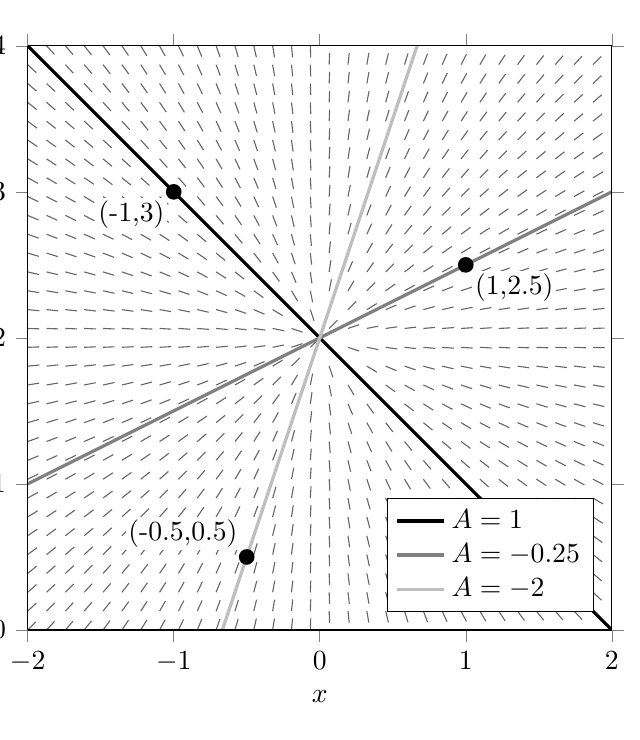
\begin{tikzpicture}[trim axis left, trim axis right] % options to centre correctly
        \def\dydx{y/x-2/x} % differential equation: dy/dx = f(x,y) => \def\dydx{f(x,y)}
        \newcommand\solution[1]{#1*x+2} % general solution with integration constant A, given by #1

        % domain and tick settings
        \def\xmin{-2} \def\xmax{2}
        \def\ymin{-0} \def\ymax{4}
        \def\xticks{\xmin,...,\xmax} % define tick marks
        \def\yticks{\ymin,...,\ymax}
        \pgfmathsetmacro\quiverScale{(\ymax-\ymin)/50}

        % #1: coordinates of node, #2: relative position of node label (can also be angle)
        \newcommand\labelledPoint[2]{\node[circle, fill, inner sep=2pt, label={[fill=white,distance=1pt,inner sep=1pt]#2:{(#1)}}] at (#1){}}

        \begin{axis}[view = {0}{90}, % set camera to point towards x-y plane
                     domain=\xmin:\xmax, y domain=\ymin:\ymax,
                     xmin=\xmin, xmax=\xmax,
                     ymin=\ymin, ymax=\ymax,
                     xlabel=$x$, ylabel=$y$,
                     xtick=\xticks, ytick=\yticks,
                     tick align=outside,
                     width=9cm, height=9cm,
                     legend pos=south east, legend cell align={left},
                     axis equal image]

            % plot unit length quivers with no head
            \addplot3[black!60, quiver={u=1/(sqrt((\dydx)^2+1)), v=(\dydx)/(sqrt((\dydx)^2+1)), scale arrows=\quiverScale}, samples=32, forget plot] (x,y,0);

            % plot initial points and corresponding solution curves
            \addplot[very thick, black!100, samples=100] plot (x,\solution{-1});
            \labelledPoint{-1,3}{below left};

            \addplot[very thick, black!50, samples=100] plot (x,\solution{0.5});
            \labelledPoint{1,2.5}{below right};

            \addplot[very thick, black!25, samples=100] plot (x,\solution{3});
            \labelledPoint{-0.5,0.5}{above left};

            % add legend, ignoring quiver plot
            \legend{$A=1$, $A=-0.25$, $A=-2$}
        \end{axis}
    \end{tikzpicture}
    \caption{Slope field of $\frac{\mathrm{d}y}{\mathrm{d}x}-\frac{y}{x}=-\frac{2}{x}$, with general solution $y(x)=Ax+2$}
\end{figure}

% Example 13-5 on page 14
\begin{figure}[hbt]
    \centering
    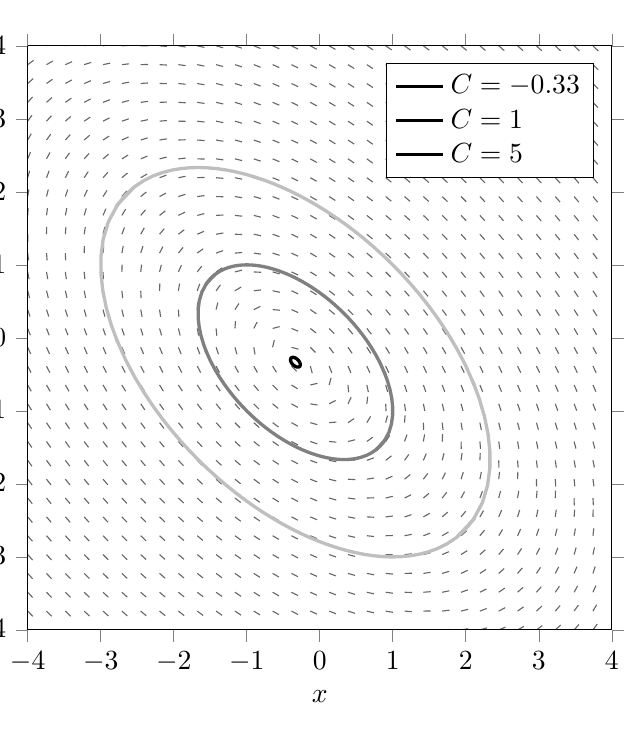
\begin{tikzpicture}[trim axis left, trim axis right] % options to centre correctly
        \def\dydx{-(2*x+y+1)/(x+2*y+1)} % differential equation: dy/dx = f(x,y) => \def\dydx{f(x,y)}

        % domain and tick settings - note domain is square, change in axis options if needed
        \def\domainMin{-4}
        \def\domainMax{4}
        \def\ticks{\domainMin,...,\domainMax} % define tick marks
        \pgfmathsetmacro\quiverScale{(\domainMax-\domainMin)/80}

        % #1: coordinates of node, #2: relative position of node label (can also be angle)
        \newcommand\labelledPoint[2]{\node[circle, fill, inner sep=2pt, label={[fill=white,distance=1pt,inner sep=1pt]#2:{(#1)}}] at (#1){}}

        % #1: integration constant c, #2: colour
        % The solution relation is x^2 + y^2 + xy + x + y = C. Rearrange for
        % y = ±f(x) and x = ±f(y), note the symmetry. Plot all 4 equations with
        % some padding to reduce overlap and regions of low resolution. All this
        % is to plot a continuous curve without using an insane amount of samples.
        % I couldn't manage to parametrise the relation.
        \newcommand\ellipse[2]{
            \pgfmathsetmacro{\lowerBound}{-1/3 * (1+2*sqrt(3*(#1)+1))}
            \pgfmathsetmacro{\upperBound}{-1/3 * (1-2*sqrt(3*(#1)+1))}
            \pgfmathsetmacro{\padding}{0.2 * (\upperBound-\lowerBound)}
            \pgfmathsetmacro{\lowerApex}{-(\lowerBound+1)/2} % apex of the ellipse (intersection with y=-(x+1)/2
            \pgfmathsetmacro{\upperApex}{-(\upperBound+1)/2}
            \addplot[very thick, #2, samples=40, domain={\lowerBound+0.2*\padding}:{\upperBound-0.2*\padding}] plot (\x,{-0.5*(\x+1)+sqrt((#1)-0.25*(\x+1)*(3*\x-1))});
            \addplot[very thick, #2, samples=40, domain={\lowerBound+0.2*\padding}:{\upperBound-0.2*\padding}] plot (\x,{-0.5*(\x+1)-sqrt((#1)-0.25*(\x+1)*(3*\x-1))});
            \addplot[very thick, #2, samples=10, domain={\lowerApex-\padding}:{\lowerApex+\padding}, variable=\y]  plot ({-0.5*(\y+1)-sqrt((#1)-0.25*(\y+1)*(3*\y-1))}, {\y});
            \addplot[very thick, #2, samples=10, domain={\upperApex-\padding}:{\upperApex+\padding}, variable=\y]  plot ({-0.5*(\y+1)+sqrt((#1)-0.25*(\y+1)*(3*\y-1))}, {\y});
        }

        \begin{axis}[view = {0}{90}, % set camera to point towards x-y plane
                     domain=\domainMin:\domainMax,
                     xmin=\domainMin, xmax=\domainMax,
                     ymin=\domainMin, ymax=\domainMax,
                     xlabel=$x$, ylabel=$y$,
                     xtick=\ticks, ytick=\ticks,
                     tick align=outside,
                     width=9cm, height=9cm,
                     legend pos=north east, legend cell align={left},
                     axis equal image]

            % plot unit length quivers with no head
            \addplot3[black!60, quiver={u=1/(sqrt((\dydx)^2+1)), v=(\dydx)/(sqrt((\dydx)^2+1)), scale arrows=\quiverScale}, samples=32, forget plot] (x,y,0);

            % solutions
            \ellipse{-0.33}{black!100}
            \ellipse{1}{black!50}
            \ellipse{5}{black!25}

            % % add legend, ignoring quiver plot
            \legend{$C=-0.33$, $C=1$, $C=5$}
        \end{axis}
    \end{tikzpicture}
    \caption{Slope field of $\frac{\mathrm{d}y}{\mathrm{d}x}=-\frac{2x+y+1}{x+2y+1}$, with general solution $x^2+y^2+xy+x+y=C\geq-\frac13$}
\end{figure}
\end{document}
